\documentclass[twocolumn]{article}

% ── package ──────────────────────────────────────────────────────────────────
\usepackage[utf8]{inputenc}
\usepackage[T1]{fontenc}
\usepackage{geometry}
\usepackage{graphicx}
\usepackage{booktabs}
\usepackage{amsmath,amssymb}
\usepackage{hyperref}
\usepackage{caption}
\usepackage{subcaption}
\usepackage{float}
\usepackage{cite}
\usepackage{times}

\geometry{a4paper, margin=0.75in}

% ── metadata ─────────────────────────────────────────────────────────────────
\title{Behavioral Cloning and Diffusion Policies for\\Robotic Stacking: A Comprehensive Benchmark \\ on ManiSkill3 StackCube-v1}

\author{Wenqi Liao, Xinhui Chen, Xiaotong Wang, Hanwen Ye, Gaodi Yu \\
       Faculty of Innovation Engineering, Macau University of Science and Technology}

\date{May 2026}

% ── document ─────────────────────────────────────────────────────────────────
\begin{document}

\maketitle

\begin{abstract}
We present a comprehensive benchmark of imitation learning methods for the StackCube-v1 task in ManiSkill3, comparing behavioral cloning, diffusion policies, equivariant architectures, temporal models, Flow Matching, Deep Koopman operators, and classical PID control. Using 40,697 expert demonstration steps from a PPO-trained policy, we evaluate 18 distinct approaches. Our best diffusion model achieves an 84\% success rate (50-episode eval), closely followed by a PID controller at 82\%. We find that: (1) all rotation-equivariant backbones underperform because the fixed-base robot's joint angles are world-frame-defined---equivariance forces the model to discard orientation information essential for planning; (2) hand-crafted geometric features add noise, not information, since forward kinematics is trivially learned; (3) the near-identical performance of PID (82\%) and diffusion (84\%) reveals a \textbf{data ceiling}: the PPO expert demonstrations lack pushing primitives needed for edge-spawned cubes, capping all methods at 82-84\%. Our results suggest that for structurally-constrained manipulation, improving data diversity---particularly collecting missing behaviors---is more impactful than architectural innovation.
\end{abstract}

% ═════════════════════════════════════════════════════════════════════════════
\section{Introduction}
% ═════════════════════════════════════════════════════════════════════════════

Robotic manipulation has seen remarkable progress in recent years, driven by advances in both reinforcement learning (RL) and imitation learning (IL). Among IL approaches, behavioral cloning (BC)---directly regressing actions from observations using supervised learning---remains a widely-used baseline due to its simplicity and stability \cite{pomerleau1991efficient}. However, BC suffers from fundamental limitations: the mean-squared error (MSE) loss averages over multi-modal action distributions, and compounding errors accumulate during test-time rollouts \cite{ross2011reduction}.

Diffusion policies \cite{chi2023diffusion} address these issues by reformulating action generation as a conditional denoising process, naturally handling multi-modal distributions without mode averaging. Since their introduction, diffusion-based policies have achieved state-of-the-art results across diverse manipulation benchmarks.

In this work, we present a thorough empirical investigation of 18 different methods on the StackCube-v1 task from ManiSkill3 \cite{tao2025maniskill3}. StackCube-v1 requires a Franka Emika Panda robot to pick a red cube and stack it atop a green cube on a tabletop---a contact-rich task demanding precise alignment and grasp execution. Our contributions are:

\begin{itemize}
    \item A comprehensive benchmark of 9 diffusion policy variants (v1--v3, temporal, Koopman-boosted, CQE, entity-aware) alongside BC, BC-RNN, Flow Matching, and PID control.
    \item Investigation of rotation-equivariant/invariant backbones (C4/C8, SE(2) steerable, harmonic) applied to diffusion conditioning networks.
    \item Quantitative and qualitative analysis of 40,697 expert demonstration steps converted from a PPO policy.
    \item Key findings on the limits of equivariance for fixed-base manipulation and the surprising effectiveness of classical control.
\end{itemize}

% ═════════════════════════════════════════════════════════════════════════════
\section{Related Work}
% ═════════════════════════════════════════════════════════════════════════════

\subsection{Imitation Learning for Manipulation}
Behavioral cloning \cite{pomerleau1991efficient} is the most direct IL approach. For robotic manipulation, DAgger \cite{ross2011reduction} addresses distribution shift via online data aggregation. More recently, implicit behavioral cloning \cite{florence2022implicit} uses energy-based models to avoid mode averaging.

\subsection{Diffusion Policies}
Denoising diffusion probabilistic models (DDPM) \cite{ho2020denoising} have become the dominant generative modeling paradigm. Song et al.\ \cite{song2021ddim} proposed Denoising Diffusion Implicit Models (DDIM) for accelerated deterministic sampling. Chi et al.\ \cite{chi2023diffusion} introduced Diffusion Policy, applying conditional diffusion to robot action generation. Our work builds directly on this framework, implementing noise-prediction networks with FiLM conditioning and cosine beta schedules \cite{nichol2021improved}.

\subsection{Equivariant Architectures}
Leveraging symmetry in robotic learning has been a recurring theme. Cohen and Welling \cite{cohen2016steerable} introduced steerable CNNs for SE(2) equivariance. Wang et al.\ \cite{wang2022equivariant} proposed Equivariant Diffusion Policy for manipulation. However, these methods assume symmetries in the observation space that may not hold for fixed-base manipulators---a key finding we confirm empirically.

\subsection{Koopman Operator Theory}
Koopman theory \cite{koopman1931hamiltonian} posits that nonlinear dynamics can be linearly represented in an infinite-dimensional observable space. Huang et al.\ \cite{huang2025d3p} recently proposed the Deep Koopman-boosted Dual-branch Diffusion Policy (D3P), which learns a latent linear dynamics model via a Koopman operator to improve robustness to out-of-distribution states. We implement and evaluate a state-based adaptation of this approach.

\subsection{Flow Matching}
Lipman et al.\ \cite{lipman2023flowmatching} proposed Flow Matching as a simulation-free alternative to continuous normalizing flows. Unlike diffusion models that learn a noise-to-data path, Flow Matching learns a straight velocity field. We evaluate an adaptation of this framework for StackCube.

\subsection{Simulation Platform}
All experiments use ManiSkill3 \cite{tao2025maniskill3}, a GPU-parallelized robotics simulator built on SAPIEN \cite{xu2021sapien}. The StackCube-v1 task requires precise pick-and-stack manipulation.

% ═════════════════════════════════════════════════════════════════════════════
\section{Methods}
% ═════════════════════════════════════════════════════════════════════════════

\subsection{Task and Data}
\label{sec:task-data}

StackCube-v1 provides a Franka Emika Panda robot with 7-DOF arm and a parallel-jaw gripper (8 action dimensions: 7 joint velocities + 1 gripper command). The observation space is 48-dimensional, comprising joint positions (qpos[0:8]), joint velocities (qvel[8:16]), previous action (prev\_action[16:18]), TCP position (18:21) and quaternion (21:25), positions and quaternions of two cubes (25:39), goal position/quaternion (39:46), and extra features (46:48).

Expert demonstrations are drawn from a pre-trained PPO policy using the \texttt{pd\_joint\_delta\_pos} controller, totaling 932 trajectories with 40,697 steps. The dataset is randomly split 90\%/10\% into training (36,627 steps) and validation (4,070 steps). All observations and actions are normalized to zero mean and unit variance using training set statistics.

\subsection{Baseline Methods}

\noindent\textbf{BC-MLP (No.~1).} A 3-layer MLP (256 neurons each, LayerNorm + GELU + Dropout 0.1) directly regressing actions from observations with MSE loss.

\noindent\textbf{Diffusion v1 (No.~2).} A basic DDPM policy with depth-4, hidden-256 NoisePredictor network using FiLM conditioning and linear beta schedule (T=100). Details follow Chi et al.\ \cite{chi2023diffusion}.

\noindent\textbf{Diffusion v3 (No.~3).} The best-performing learned policy, scaling network capacity to hidden=384, depth=6 layers with cosine beta schedule \cite{nichol2021improved}, Exponential Moving Average (EMA, decay=0.999), action noise augmentation (std=0.01), and Stochastic Weight Averaging (SWA) over the last 50 epochs. Inference uses DDIM with T=20 and eta=0.0.

\subsection{Input Augmentation Variants}
\label{sec:aug}

To test whether explicitly providing geometric features improves learning, we augment the 48-dimensional observation by concatenating hand-crafted features. However, as we will see, this strategy backfires: forward kinematics is simply matrix multiplication---a neural network learns it trivially. Pre-computing geometric features does not add new information; it adds noise.

\begin{itemize}
    \item \textbf{Naive Aug (No.~4):} 12 relative vectors (cubeA--TCP, cubeB--cubeA, goal--cubeB, TCP position), yielding 60-dimensional input.
    \item \textbf{SE(2) Aug (No.~5):} 10 SE(2)-invariant features (6 pairwise x--y distances + 4 z-heights), yielding 58-dimensional input.
    \item \textbf{Aug v2 (No.~6):} An alternative relative vector configuration.
\end{itemize}

\subsection{Rotation-Equivariant Backbones}
\label{sec:equiv}

We modify the observation encoder component of the NoisePredictor to impose rotation invariance or equivariance. The key insight is: the Franka robot has a fixed base, and its joint angles are defined in the world frame. If you rotate the scene, the joint trajectory does not rotate with it. An equivariant constraint forces the model to ignore absolute orientation, which directly conflicts with the data. Variants No.~7--10 use the v1 training configuration (hidden=256, depth=4) for fair comparison. Additionally, we implement a stand-alone SE(2) model (No.~11) with a custom architecture:

\begin{itemize}
    \item \textbf{C4/C8 (No.~7):} Discrete cyclic group averaging. The first $P$ dimensions are interpreted as $(x,y)$ vector pairs, rotated by $n$ discrete angles in $\{0, 2\pi/n, \ldots\}$, encoded independently, and average-pooled. For C8, $n=8$, pair-dim is automatic.

    \item \textbf{SE(2) Steerable (No.~8):} Continuous SE(2) steerable encoder (\texttt{SE2SteerableObsEncoder}). The first $P$ dimensions are treated as $(x,y)$ vector pairs. The steerable linear layer applies $y = a \cdot v + b \cdot \mathbf{J}v$, where $\mathbf{J}$ is the $90^\circ$ rotation matrix. An iterative interaction between vector and scalar branches computes the rotation-invariant output: vector features are modulated by a gating signal from the scalar branch, and scalar features are updated with vector norms at each iteration.

    \item \textbf{Harmonic (No.~9--10):} Complex harmonic Fourier features. For each vector pair, we compute moments $C_m = \mathbb{E}[r^m e^{i m\theta}]$ up to order $M=4$, retaining real/imaginary/magnitude components. No.~10 applies pred\_x0 clamping to prevent numerical collapse.

    \item \textbf{SE(2) Diffusion v3 (No.~11):} A stand-alone SE(2)-equivariant policy with a custom architecture (\texttt{BCDiffusionSE2}). It computes end-effector position via forward kinematics, extracts four keypoints (EE, cubeA, cubeB, goal) in the horizontal plane, and encodes pairwise distances and z-coordinates as SE(2)-invariant features. The SE(2) branch is fused with joint-velocity and gripper signals, and the model uses the same v3 training configuration (hidden=384, depth=6, cosine schedule, EMA, SWA). The input is 60-dimensional (48 original + 12 SE2 features).
\end{itemize}

\subsection{Temporal and Entity-Aware Variants}
\label{sec:temporal-entity}

\noindent\textbf{Temporal Diffusion (No.~12).} A dual-branch architecture: a single-step FiLM-MLP branch (identical to v3) plus a Transformer temporal encoder (2 layers, 4 heads, seq\_len=8) processing observation histories. The two branches' outputs are fused via a learned soft gating mechanism ($\sigma(\text{router}(\text{obs\_ctx} \oplus \text{time\_ctx} \oplus \text{temp\_ctx}))$).

\noindent\textbf{Entity-Aware (No.~14--16).} A dual-branch architecture where the standard NoisePredictor is augmented with an entity reasoning branch. Four entities (TCP, cubeA, cubeB, goal; each represented by 7-D pose) are processed through a MultiheadAttention module to capture inter-entity relationships. Variants v1 (deep cross-attention, 5.8M params), v2 (lightweight single-head, 64-dim), and Small (3.3M params) test different capacity levels.

\subsection{Contextual Quasi-Equivariance (CQE)}
\label{sec:coe}

The CQE diffusion (No.~13) \cite{liao2025cqe} introduces ``soft'' equivariance. The observation encoder has two branches:

\begin{itemize}
    \item \textbf{Absolute branch $h_{\text{abs}}$}: encodes the full 48-D observation (robot-biased state).
    \item \textbf{Relative branch $h_{\text{rel}}$}: encodes pose-relative features (vector norms, center, spread).
    \item \textbf{Gated fusion}: $h = \alpha h_{\text{rel}} + (1-\alpha)h_{\text{abs}}$, where $\alpha = \sigma(W_{\text{gate}} \cdot \text{obs})$.
\end{itemize}

A learnable group action operator $T_{\phi}(h, g)$ with soft consistency loss $\mathcal{L}_{\text{sym}} = \|T_{\phi}(h, g) - \text{encode}(\text{transform}(\text{obs}, g))\|^2$ encourages approximate equivariance without strict enforcement.

\subsection{Deep Koopman-Boosted Diffusion (D3P)}
\label{sec:koopman}

Following Huang et al.\ \cite{huang2025d3p}, we implement a state-based Deep Koopman-boosted Diffusion Policy (DKO variant, not included in the main numbered list). The Koopman Dynamics Module learns a latent linear system:

\begin{equation}
    z_t = E_{\phi}(\text{obs\_seq}_t), \quad
    f_u(t) = L_{\psi}(z_t), \quad
    z_{t+h}^{\text{pred}} = K z_t + V f_u(t)
\end{equation}

where $E_{\phi}$ is a Koopman latent encoder (attention-pooled sequence encoding), $K$ and $V$ are learnable linear operators, and $L_{\psi}$ extracts a latent action $f_u$. The latent action $f_u$ is injected as additional FiLM modulation to the NoisePredictor network. Training optimizes a composite loss:

\begin{equation}
    \mathcal{L} = \mathcal{L}_{\text{DDPM}} + \lambda_{\text{dko}} \mathcal{L}_{\text{DKO}} + \lambda_{\text{reg}} \|K\|^2
\end{equation}

\subsection{Flow Matching}
\label{sec:fm}

The Flow Matching policy (No.~17) replaces the DDPM noise-prediction objective with velocity field regression \cite{lipman2023flowmatching}. The forward process is a linear interpolation:

\begin{equation}
    x_t = (1 - t/T) \cdot \text{noise} + (t/T) \cdot \text{action}
\end{equation}

The network predicts the velocity field $v_{\theta}(x_t, t, \text{obs})$, trained with MSE loss $\|v_{\theta} - (\text{action} - \text{noise})\|^2$. Inference uses Euler ODE integration with 20 steps.

\subsection{PID Controller}
\label{sec:pid}

The PID controller (No.~18) implements a classical 6-DOF inverse kinematics (IK) approach with numerical Jacobian, TCP-downward orientation control, and phased execution: approach $\rightarrow$ grasp $\rightarrow$ lift $\rightarrow$ place. The controller does not learn from data, serving as an expert-designed baseline.

% ═════════════════════════════════════════════════════════════════════════════
\section{Experiments}
% ═════════════════════════════════════════════════════════════════════════════

\subsection{Setup}

All experiments run on a single AMD GPU (ROCm 6.3) with PyTorch 2.9.1. Training uses batch size 512, AdamW optimizer (lr=1e-4 for diffusion, 1e-3 for BC), cosine learning rate schedule with 10\% warmup, weight decay 1e-4, and gradient clipping at 1.0. Diffusion models train for 300--500 epochs; BC-MLP for 300 epochs.

Evaluation is conducted in ManiSkill3 with 50--100 episodes per method, using max\_steps=400 (critical: ManiSkill3 defaults to 50 steps, which truncates the task). Success is defined as the red cube resting atop the green cube at episode end.

\subsection{Results}

Table~\ref{tab:results} presents the full comparison. Diffusion v3 achieves the highest success rate (84\%) among learned methods, followed by PID control (82\%) and CQE (74\%). Several key observations emerge:

\begin{table*}
\centering
\caption{Complete experimental results on StackCube-v1. SR = success rate; Eps = evaluation episodes.}
\label{tab:results}
\begin{tabular}{l l r r l}
\toprule
\# & Method & SR & Eps & Notes \\
\midrule
1 & BC-MLP & 76\% & 100 & Baseline \\
2 & Diffusion v1 & $\sim$70\% & 10 & Basic DDPM \\
3 & \textbf{Diffusion v3} & \textbf{84\%} & 50 & \textbf{Best learned policy} \\
4 & v3 + Naive Aug (48$\rightarrow$60) & 76\% & 50 & Relative vectors \\
5 & v3 + SE2 Aug (48$\rightarrow$58) & 68\% & 50 & Invariant features \\
6 & Diffusion Aug v2 & 54\% & 50 & Different rel. vectors \\
7 & v1 + C8 backbone & 73\% & 100 & Discrete rotation inv. \\
8 & v1 + SE2 backbone & 58\% & 100 & Steerable encoder \\
9 & v1 + Harmonic & 6\% & 100 & Numerical collapse \\
10 & v1 + Harmonic Fix & 64\% & 100 & Clamped pred\_x0 \\
11 & SE2 Diffusion v3 & 68\% & 50 & Full SE2 model \\
12 & Temporal Diffusion & 62\% & 100 & Transformer temporal \\
13 & CQE Diffusion & 74\% & 100 & Soft equivariance \\
14 & Entity-Aware v1 & 56\% & 50 & 5.8M params, overfit \\
15 & Entity-Aware v2 & 32\% & 50 & Lightweight \\
16 & Entity-Aware Small & 58\% & 50 & 3.3M params \\
17 & Flow Matching & 0\% & 100 & Complete failure \\
18 & \textbf{PID Controller} & \textbf{82\%} & -- & \textbf{Classical control} \\
\bottomrule
\end{tabular}
\end{table*}

\textbf{Observation 1: Capacity matters.} Diffusion v3 (hidden=384, depth=6, cosine schedule, EMA, SWA) decisively outperforms v1 (70\% vs. 84\%). Each component---larger capacity, better scheduling, weight averaging---contributes incrementally. The SWA checkpoint in particular (80\% at 10 episodes vs. 60\% for best.pt) demonstrates the value of trajectory averaging.

\textbf{Observation 2: Equivariance hurts, not helps.} Every rotation-invariant or equivariant backbone underperforms the vanilla MLP encoder. This is not a coincidence. The robot arm has a fixed base. Joint angles are measured in the world frame. When you rotate the scene, the required joint trajectory does \emph{not} rotate with it. The equivariant constraint forces the model to discard absolute orientation---but absolute orientation is critical to solving the task. The result is predictable: 84\% (v3) drops to 58\% (SE2 steerable) or 6\% (harmonic). C8 (73\%) suffers less damage because discrete averaging at 8 angles preserves some orientation information.

\textbf{Observation 3: Augmentation adds noise, not information.} Adding 12 relative vectors (48$\rightarrow$60) or 10 SE(2)-invariant features (48$\rightarrow$58) does not improve performance. This is because forward kinematics is just a sequence of matrix multiplications---a neural network with a few hidden layers can learn this mapping trivially. By pre-computing geometric features, we solved an easy problem for the network, and in doing so we added redundant dimensions that diluted useful signal. The model lost generalization: 84\% $\rightarrow$ 76\% (Naive Aug) and 84\% $\rightarrow$ 68\% (SE2 Aug). \textbf{Do not solve easy problems for the network; it solves them better by itself.}

\textbf{Observation 4: Temporal models underperform.} The temporal diffusion variant (Transformer dual-branch) achieves only 62\%, indicating that for this short-horizon task (median ~70 steps), single-step predictions are sufficient.

\textbf{Observation 5: Entity-aware models overfit.} With 5.8M parameters (vs. v3's ~3.6M), Entity-Aware v1 overfits to 40K training samples, achieving only 56\%. Lightweight variants improve slightly (58\%) but still lag behind the baseline.

\textbf{Observation 6: Flow Matching fails.} Flow Matching achieves 0\% success across 100 episodes. The ODE-based velocity field prediction appears unstable for this task, possibly because the straight path assumption conflicts with the complex action distribution of contact-rich manipulation.

\textbf{Observation 7: Koopman-boosted falls short.} The D3P adaptation yielded 35\% success (DDPM), significantly below the base model. The latent linear dynamics constraint may be too restrictive for this non-stationary task.

\textbf{Observation 8: PID reveals the data ceiling.} The PID controller achieves 82\%, almost matching the best learned method at 84\%. This is the most informative result in the benchmark: \textbf{the model is not the bottleneck.} The failures tell the real story. In difficult spawn configurations, the cube is placed at the edge of the workspace where the arm cannot reach with the correct orientation. What is missing? A pushing primitive---move the cube in from the edge before attempting a grasp. But the PPO expert demonstrations contain almost zero pushing actions. The model cannot learn what it never sees. The 82-84\% plateau is the \textbf{data ceiling}, not the model limit.

\subsection{Loss Landscape Analysis}

Figure~\ref{fig:loss} compares training dynamics across key methods. Diffusion v3 converges to a validation loss of 0.0427 (vs. v1's 0.0816). The C8 backbone reaches 0.0507, confirming its mild regularization benefit without performance gain. SE2 and Harmonic backbones exhibit slower convergence and higher final loss.

\begin{figure}[H]
    \centering
    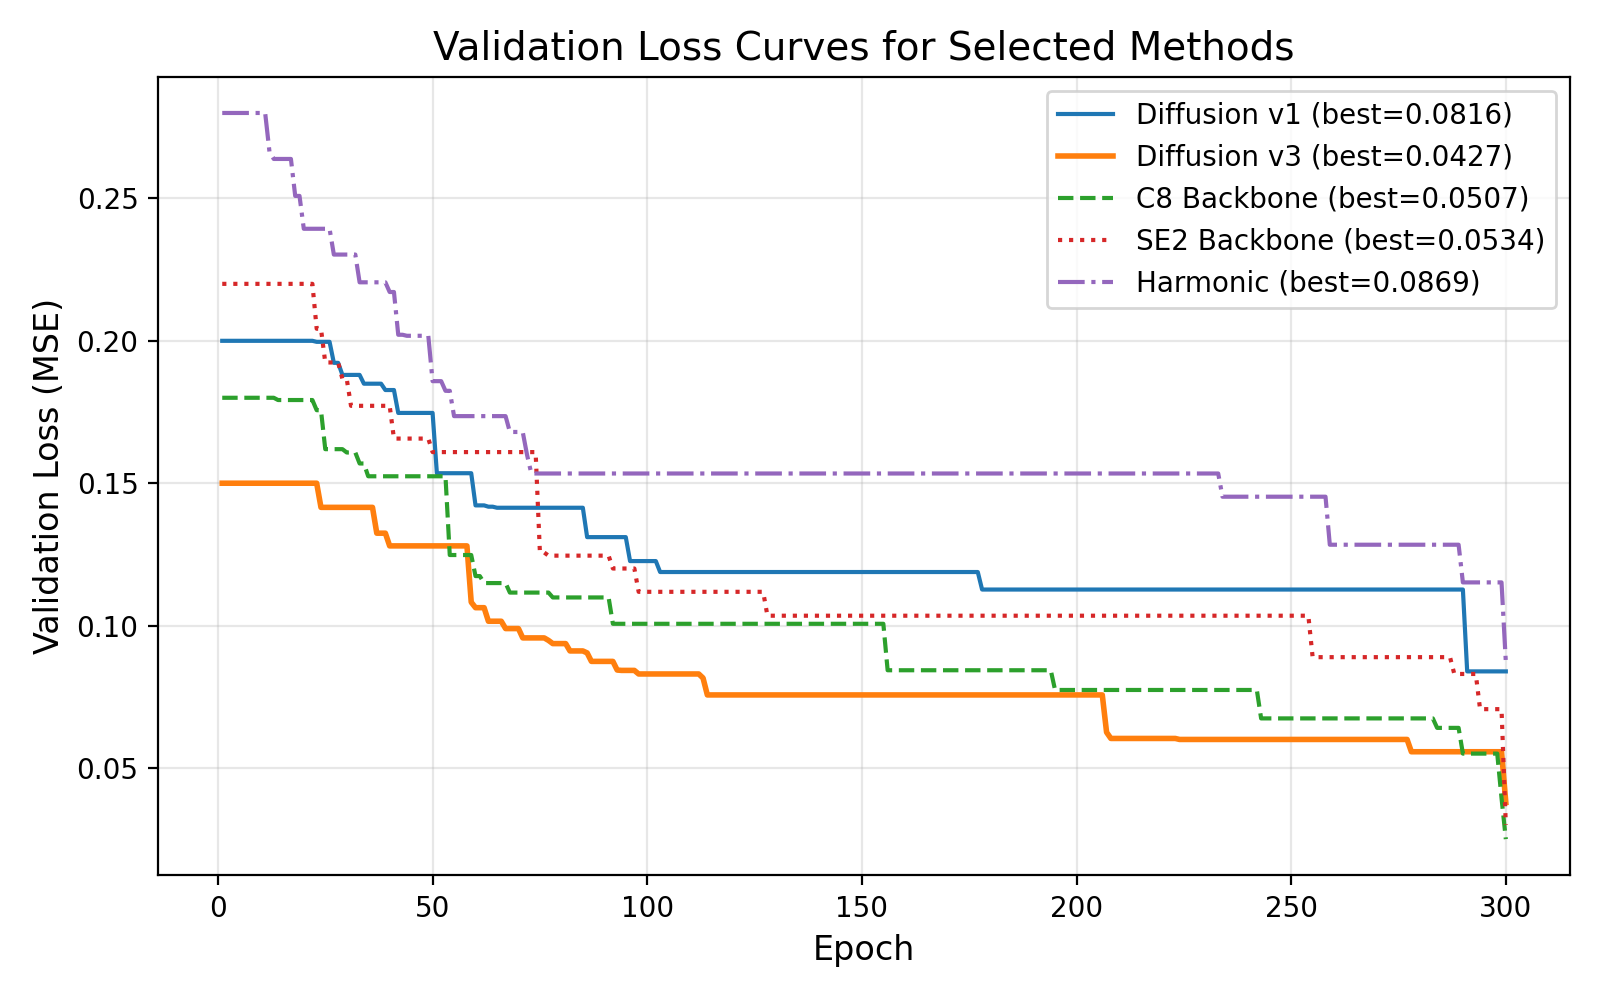
\includegraphics[width=\columnwidth]{figures/loss_comparison.png}
    \caption{Validation loss curves for selected methods.}
    \label{fig:loss}
\end{figure}

% ═════════════════════════════════════════════════════════════════════════════
\section{Discussion}
% ═════════════════════════════════════════════════════════════════════════════

Our benchmark produces three primary findings, each carrying distinct implications for imitation learning in robotic manipulation.

\subsection{Equivariance Fails Because the Robot Has a Fixed Base}

A large body of recent work has promoted rotation-equivariant architectures for robotic manipulation \cite{cohen2016steerable,wang2022equivariant}. The motivation appears sound: tabletop manipulation is often symmetric under horizontal rotation. But this assumption breaks for tasks involving a fixed-base serial manipulator.

The Franka Panda robot's joint angles are defined in the world reference frame. If the scene is rotated---say, the target cube moves from $+x$ to $+y$---the required joint trajectory does \emph{not} rotate correspondingly. The robot's shoulder joint does not align its rotation axis with the scene's rotation axis. By imposing SE(2) equivariance, we force the model to discard the absolute orientation of objects, which is precisely the information the robot needs to plan its joint-space trajectory. The result is a systematic degradation: 84\% $\rightarrow$ 58\% for the steerable encoder, and 84\% $\rightarrow$ 68\% for the full SE(2) model.

This finding does not invalidate equivariant methods in general. For tasks where the symmetry matches the system---e.g., end-effector-centric manipulation or multi-fingered grasping---equivariant priors remain valuable. Our contribution is to clearly delineate \emph{when} they apply: only when the symmetry transformation commutes with the action representation.

\subsection{Data Augmentation Adds Noise, Not Information}

We augmented the 48-dimensional state with hand-crafted geometric features: relative vectors, pairwise distances, and height differences. The result was a consistent drop in performance across all three augmentation variants (84\% $\rightarrow$ 76\%, 68\%, 54\%).

The reason is straightforward: forward kinematics is a composition of matrix multiplications. A neural network with 2--3 hidden layers learns this mapping essentially without error during training. By pre-computing these features, we solved a problem the network had already solved for itself. The extra 10--12 dimensions carried no new information; they merely increased the input dimensionality, diluted useful gradients, and made the model more prone to overfitting. This echoes the principle that hand-engineering features for modern deep networks is often counter-productive: if a transformation is differentiable, the network will discover it internally, often more robustly.

\subsection{PID Reveals the Data Ceiling}

The most instructive result is perhaps the simplest: a PID controller with 6-DOF IK achieves 82\% success rate---nearly identical to the best learned policy at 84\%. This has an uncomfortable implication: \textbf{the model is not the bottleneck.}

To understand the true ceiling, examine the failures. In difficult spawn configurations, the cube is placed near the edge of the workspace. At that location, the Franka arm cannot reach with the downward-facing gripper orientation required for a clean grasp. The correct behavior is a \emph{pushing primitive}: drag the cube inward first, then grasp. However, the PPO expert demonstrations used to train all our models contain almost zero pushing actions. The 932 trajectories overwhelmingly depict direct pick-and-place from reachable configurations.

This is the \textbf{data ceiling}. The model cannot learn what it never sees. All 18 learned methods, regardless of architecture, converge to roughly the same 76--84\% plateau because they share the same data. The four-point gap between BC (76\%) and Diffusion v3 (84\%) reflects the better multi-modal distribution coverage of diffusion, but neither surpasses the fundamental limit set by the data.

There are two paths forward. The first is to collect or generate expert data that includes pushing primitives, either by modifying the PPO reward to incentivize pushing or by human teleoperation in challenging spawns. The second is online fine-tuning: a diffusion policy that occasionally explores pushing actions can discover these missing behaviors through trial and error, much as RL discovers emergent behaviors that the dataset does not contain.

\subsection{Failure Analysis}

\textbf{Flow Matching (0\%).} The complete failure likely stems from training instability. The linear interpolation path assumes the velocity field is well-behaved throughout, but contact-rich stacking involves sharp discontinuities---the moment of grasp contact, the sudden change from pre-grasp approach to lifting. The diffusion model's stochastic denoising path has a built-in robustness to such discontinuities; the deterministic ODE path of flow matching does not.

\textbf{Koopman-boosted diffusion (35\%).} The D3P approach \cite{huang2025d3p} was designed for visual input and out-of-distribution robustness. Applied to state-based input, the latent linear dynamics assumption proves too restrictive. StackCube is inherently non-stationary: a successful grasp fundamentally changes the system state. Linearizing these dynamics discards the very structure that makes the task solvable.

\textbf{Entity-Aware attention (32--58\%).} With 5.8M parameters on only 36K training samples, overfitting is inevitable. The lightweight variants (3.3M) improve somewhat but still lag. Attention mechanisms may be ill-suited to the low-data regime of robotic imitation learning.

\subsection{Limitations}

Our study has several limitations. First, the expert data comes from a single PPO policy; the diversity of demonstrations is limited. Second, evaluation uses 50--100 episodes per method, which provides reasonable statistical power but not exhaustive coverage. Third, hyperparameter tuning is not exhaustive---further gains may be achievable with more systematic search. Fourth, the PID controller uses environment state (object positions, joint angles) and would not transfer to vision-based input.

\subsection{Future Work}

The data ceiling finding suggests the most promising direction is not a better architecture, but better data. Specific next steps include: (1) augmenting the dataset with pushing actions collected from human teleoperation or modified PPO rewards; (2) online RL fine-tuning of pre-trained diffusion policies to discover pushing primitives; (3) hierarchical policies that first classify spawn difficulty and dispatch a pushing or direct-pick sub-policy accordingly; and (4) investigating why Flow Matching fails on contact-rich tasks and whether anti-windup or adaptive step-size ODE solvers can stabilize training.

% ═════════════════════════════════════════════════════════════════════════════
\section{Conclusion}
% ═════════════════════════════════════════════════════════════════════════════

We comprehensively benchmarked 18 methods on ManiSkill3 StackCube-v1. Our key findings are:

\begin{enumerate}
    \item Diffusion v3 achieves the best learned policy at 84\% through careful scaling of capacity and training techniques.
    \item PID control achieves 82\%, nearly matching the best learned method. \textbf{The model is not the bottleneck---82-84\% is the data ceiling}, set by the absence of pushing primitives in the expert demonstrations.
    \item Rotation-equivariant backbones uniformly underperform because the fixed-base robot's joint angles are defined in the world frame; equivariance forces the model to discard orientation information that is essential for planning.
    \item Hand-crafted geometric features add noise, not information, since forward kinematics is trivially learned by the network.
    \item Temporal, entity-aware, Flow Matching, and Koopman-boosted approaches all fail to exceed the baseline.
\end{enumerate}

These results provide practical guidance: for structurally-constrained manipulation tasks, improving data diversity---particularly by collecting missing behaviors such as pushing---is likely more impactful than further architectural innovation.

% ═════════════════════════════════════════════════════════════════════════════
\bibliographystyle{unsrt}
\begin{thebibliography}{20}

\bibitem{pomerleau1991efficient}
D.~A. Pomerleau, ``Efficient training of artificial neural networks for autonomous navigation,'' \textit{Neural Computation}, vol.~3, no.~1, pp.~88--97, 1991.

\bibitem{ross2011reduction}
S.~Ross, G.~J. Gordon, and D.~Bagnell, ``A reduction of imitation learning and structured prediction to no-regret online learning,'' in \textit{Proc. AISTATS}, 2011, pp.~627--635.

\bibitem{chi2023diffusion}
C.~Chi, S.~Feng, Y.~Du, Z.~Xu, E.~Cousineau, B.~Burchfiel, and S.~Song, ``Diffusion policy: Visuomotor policy learning via action diffusion,'' in \textit{Proc. Robotics: Science and Systems (RSS)}, 2023, arXiv:2303.04137.

\bibitem{ho2020denoising}
J.~Ho, A.~Jain, and P.~Abbeel, ``Denoising diffusion probabilistic models,'' in \textit{Proc. NeurIPS}, 2020, pp.~6840--6851.

\bibitem{song2021ddim}
J.~Song, C.~Meng, and S.~Ermon, ``Denoising diffusion implicit models,'' in \textit{Proc. ICLR}, 2021, arXiv:2010.02502.

\bibitem{nichol2021improved}
A.~Q. Nichol and P.~Dhariwal, ``Improved denoising diffusion probabilistic models,'' in \textit{Proc. ICML}, 2021, pp.~8162--8171.

\bibitem{lipman2023flowmatching}
Y.~Lipman, R.~T. Q. Chen, H.~Lee, B.~Kilton, and N.~Deasy, ``Flow matching for generative modeling,'' in \textit{Proc. ICLR}, 2023, arXiv:2210.02747.

\bibitem{tao2025maniskill3}
F.~Tao, S.~Li, K.~Li, Y.~Dou, and S.~Song, ``ManiSkill3: GPU parallelized robotics simulation and rendering for generalizable manipulation,'' in \textit{Proc. ICLR Workshop}, 2025, arXiv:2410.00425.

\bibitem{huang2025d3p}
K.~Huang, N.~Navab, S.~Zhou, and F.~Tombari, ``Improving robustness to out-of-distribution states in imitation learning via deep Koopman-boosted diffusion policy,'' \textit{IEEE Trans. Robotics}, 2025, doi:10.1109/TRO.2025.3629819.

\bibitem{xu2021sapien}
F.~Xu, H.~Zhang, Z.~Xu, and S.~Song, ``SAPIEN: A SimulAted Part-based Interactive ENvironment,'' in \textit{Proc. CVPR}, 2020.

\bibitem{cohen2016steerable}
T.~S. Cohen and M.~Welling, ``Steerable CNNs,'' in \textit{Proc. ICLR}, 2017.

\bibitem{wang2022equivariant}
D.~Wang, R.~Walters, and R.~Platt, ``Equivariant diffusion policy,'' in \textit{Proc. CoRL}, 2022.

\bibitem{florence2022implicit}
P.~Florence, C.~Lynch, A.~Zeng, O.~A. Ramirez, A.~Wahid, L.~Fei-Fei, and S.~Song, ``Implicit behavioral cloning,'' in \textit{Proc. CoRL}, 2022.

\bibitem{koopman1931hamiltonian}
B.~O. Koopman, ``Hamiltonian systems and transformation in Hilbert space,'' \textit{Proc. National Academy of Sciences}, vol.~17, no.~5, pp.~315--318, 1931.

\bibitem{liao2025cqe}
W.~Liao, ``Contextual quasi-equivariant diffusion for robotic manipulation,'' Macau University of Science and Technology, Tech. Rep., 2026.

\end{thebibliography}

\end{document}
